\chapter{HomeDS - Server}
\section{Einleitung}\label{sec:einleitung}
Im Rahmen der Diplomarbeit wird neben dem XIBO-Server ein eigen Programmierter Java Enterprise Edition Server eingesetzt. Aufgrund der hohen Komplexität des Signage-Servers aber relativ dünn dokumentierten API-Schnittstellen und begrenzten technischen Möglichkeiten muss ein eigen programmierter Server eingesetzt werden. Dieser wird die Kommunikation vom Signage Server zur Android App erleichtern.  
 
\section{Java Enterprise Edition}\label{sec:javaee}
Java Platform, Enterprise Edition, oder abgekürzt auch Java EE ist die technische nähere Beschreibung einer Softwarearchitektur die Java Programmierte Anwendungen ausführt.
(weiter ausführen)

QUELLE: https://de.Wikipedia.org/wiki/Java_Platform,_Enterprise_Edition
 
\section{Anforderungen an den HomeDS Server}\label{sec:homeds}
Der JavaEE Server soll die verschiedenen komplizierten Abläufe des XIBO-Servers vereinfachen. Die verschiedenen Zugriffe mittels REST die eigentlich direkt auf den XIBO laufen sollen werden über den JavaEE Server verwaltet. Dies hat insofern Vorteile da die komplizierten und meist mit viel Aufwand verknüpften Authentifizierungen wegfallen. Somit können ohne Probleme neue Funktionen hinzugefügt werden und ohne Probleme an neue Anforderungen angepasst werden.
 
\section{Funktionen des HomeDS Server}\label{sec:homedsfunction}
Der JavaEE Server verfügt über eine eigene MySQL Datenbank. Diese wird gebraucht um die "DataSets" aus dem Signage-Server zwischen zu speichern. Dies ist insofern erforderlich da die Aufgabenstellung erfordert die Datensätze entweder nur ab einem bestimmten Datum im Layout anzuzeigen oder bis zu einem bestimmten Datum diese angezeigt werden dürfen. 
 
\section{DataSet mit Ablaufdatum}\label{sec:datasetexpiredate}
Einer der wichtigsten Funktionen des Servers ist das hinzufügen, ändern und löschen vom DataSet. Da der Digital Signage Server über keine Felder wie Start- und Enddatum verfügen.

Die Logik ist simple der Benutzer kann Start- und Enddatum eingeben für jeden einzelnen DataSet eingeben. Und erst wenn das Datum genau in diesem Zeitintervall inklusive den Grenzen liegt wird das DataSet an den Xibo mittels API-Schnittstelle weitergegeben. 

\begin{lstlisting}
if (dataset.isActive() == false && (dataset.getFromDate().minusDays(1)
        .isBefore(LocalDate.now()))) {
    try {
        //if succesfull added then set active true and add id
        if ((id=dataSetApi.addDataSetField(dataset)) > 0) {
            dataset.setDataRowId(id);
            dataset.setActive(true);
            dataSetFieldFacade.save(dataset);
        }
    } catch (NoConnectionException e) {
        // Catch Exception
    }
}
\end{lstlisting}

Die Überprüfung ob die DataSets aus der Server-Datenbank im Zeitintervall liegen wird mittels eines "TimeSchedule" jeden Tag um 01:00 Uhr durchgeführt. Falls dieser dann im Intervall liegt wird der DataSet an den XIBO Signage Server gesendet. Diese Überprüfung beinhaltet auch das FromDate dies löscht bei überschreiten des Bis-Datums das DataSet aus dem Digital Signage heraus. 

Die Überprüfung ob das Startdatum heute oder vor dem heutigem Datum wird mithilfe der Java Annotation @Schedule realisiert. (siehe Codeausschnitt) 


 
\begin{enumerate}
  \item {\em :} Mit der Kalender Funktion kann eingetragen werden zu welchen Zeitpunkt welcher Inhalt auf welchem Bildschirm angezeigt werden soll. In dem Xibo-Kalender werden auch bereits eingetragene Aktivitäten angezeigt.
 
\begin{calendar}
  \centering
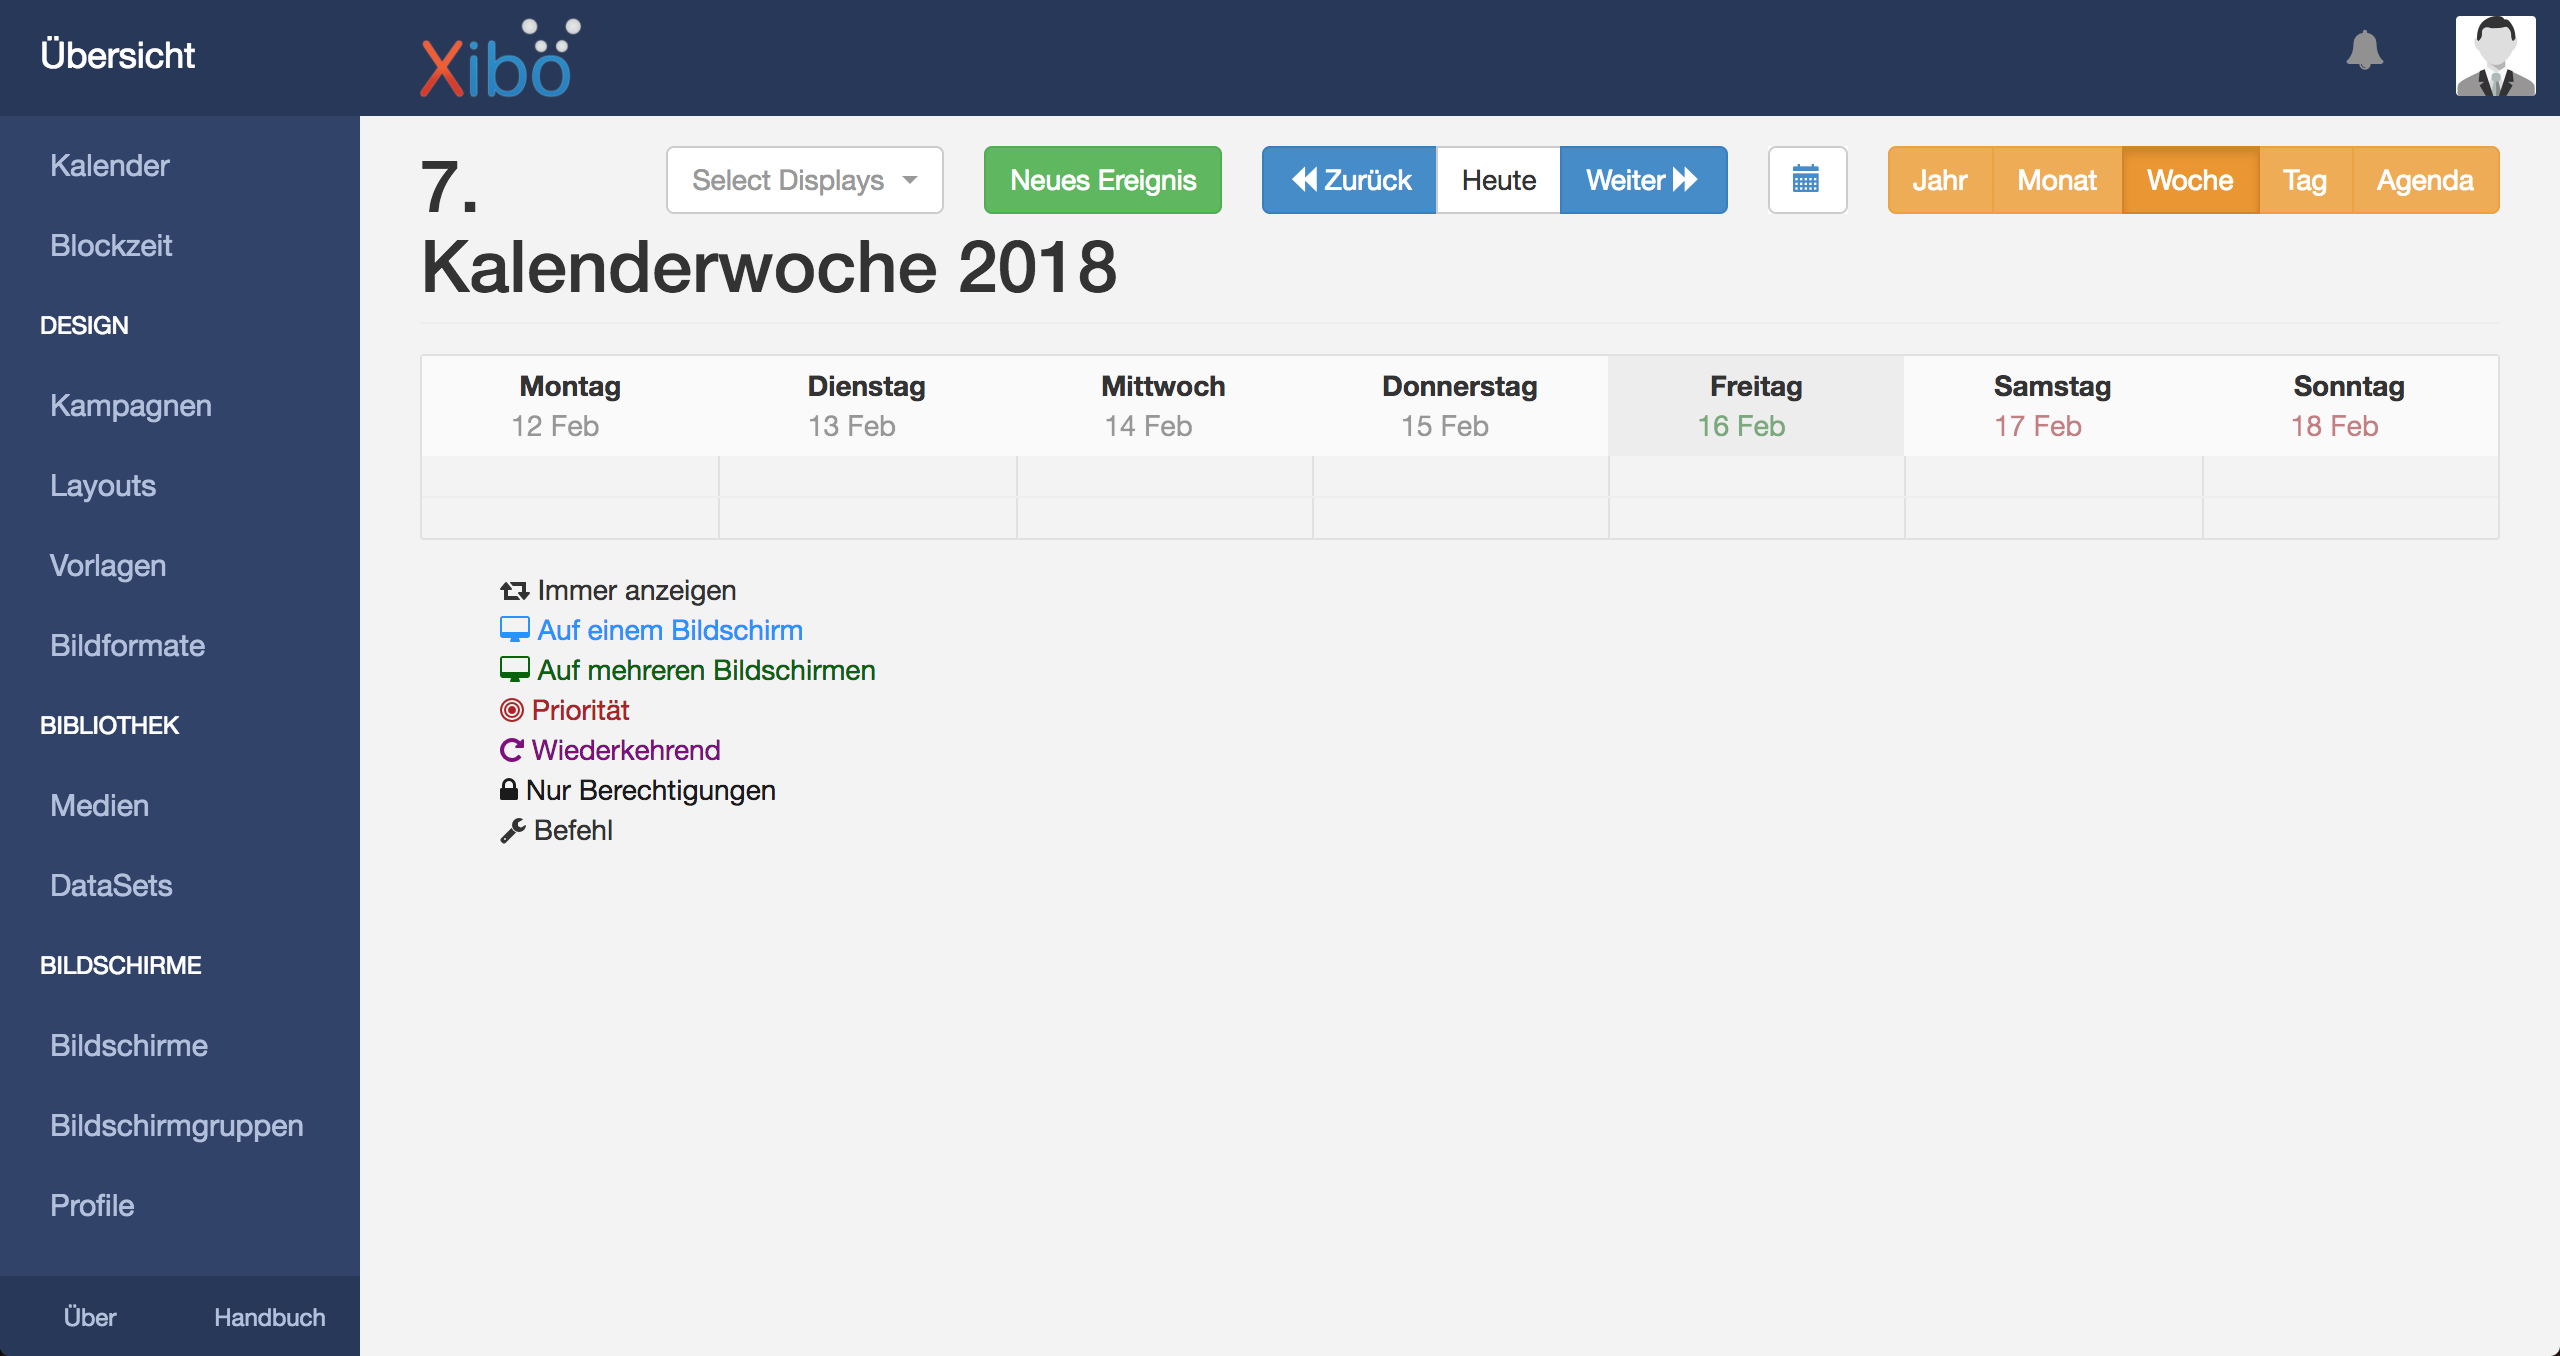
\includegraphics[width=1\textwidth]{images/xibo-basics-calendar}
  \label{Calendar}
\end{calendar}  
  
  \item {\em Layouts:} 
  Die Layout Funktion ist einer der wichtigsten Komponenten des Signage Systems es beschäftigt sich mit dem designen der Inhalte. Auf diese Funktion kommen wir noch einmal zurück
  
  \item {\em Bibliothek:} 
  Die Bibliothek Funktion ist zuständig für das Verwalten der Medien. Hier können Sie verschiedene Dateien hochladen.  Diese Medien können dann in Layouts eingebunden und angezeigt werden.
  
  \item {\em Benutzer:} 
  Im Menüpunkt Benutzer können neue Benutzer angelegt werden und bereits bestehende bearbeitet oder gelöscht werden. Dabei gibt es auch ein Rechte-System. Es könne auch Datenmengen Begrenzungen pro Benutzer eingestellt werden.
  
  \item {\em Einstellungen:} 
  Der Menöpunkt Einstellung gibt dem Nutzer die Möglichkeit verschiedene Optionen einzustellen. So sind zum Beispiel die richtige Zeitzone, E-Mail Benachrichtigungen wichtige Einstellungen die für ein Einwandfreies funktionieren des Xibo-Servers zuständig wichtig sind.
\end{enumerate}
 
\section{Designen mit XIBO}\label{sec:designexibo}
Beim Designen von einem neuen Layout im XIBO muss zuerst die Bildschirm auflösung ausgewählt werden. Und dem Layout ein passender Name zugewiesen werden sowie optional auch eine Beschreibung. 
 
\textbf{Layout Maske}
 
\begin{calendar}
  \centering
1 file change in working directory
View change
commit:c95ae5
WIP on master: Auto stash before merge of "master" and "origin/master"
